\label{ch:laravel}
Wanneer we kijken naar de tekortkomingen die Drupal heeft, is het geen overbodige investering om op zoek te gaan naar een alternatief dat deze tekortkomingen kan overbruggen. In de zoektocht naar dit alternatief zijn er verschillende criteria waar we rekening mee dienen te houden. Zowel Drupal als Laravel hebben een gelijklopend applicatieplatform en doelpubliek. Bovendien gebruiken beide PHP. 

\section{Wat is Laravel?}
Laravel is een MVC framework geschreven in PHP, om webapplicaties te ontwikkelen. Dit framework is ontworpen om de kwaliteit van de te ontwikkelen software te verbeteren. Door de duidelijke, vooruitstrevende syntax en kernfuncties bespaart dit veel tijd bij het voltooien van een applicatie. De filosofie van Laravel opteert voor conventie over configuratie. Het komt erop neer dat je meestal je doel bereikt met minder code waarbij ernaar gestreefd wordt het midden te houden tussen minimalistisch en functioneel. Het spreekt voor zich dat het begrijpen van leesbare code eenvoudiger is. Het stuurprogramma geeft je de vrijheid om op eenvoudige wijze aanpassingen door te voeren aan caching-, session-, database- en authenticatiefuncties. 
\newline\newline
Laravel maakt gebruik van de command-line-interface Artisan. Met deze tool is het mogelijk om als ontwikkelaar testen, migraties en periodieke taken uit te voeren. 

\section{Trending}
Onderstaande link geeft een overzicht van Google Search Words die trending zijn over verloop van tijd. We lijsten de meest populaire PHP frameworks op en zien duidelijk dat Laravel de leiding neemt. Laravel heeft het grootste relatieve aandeel, alsook de sterkste stijging. 
\newline\newline\noindent

\begin{figure}[!ht]
  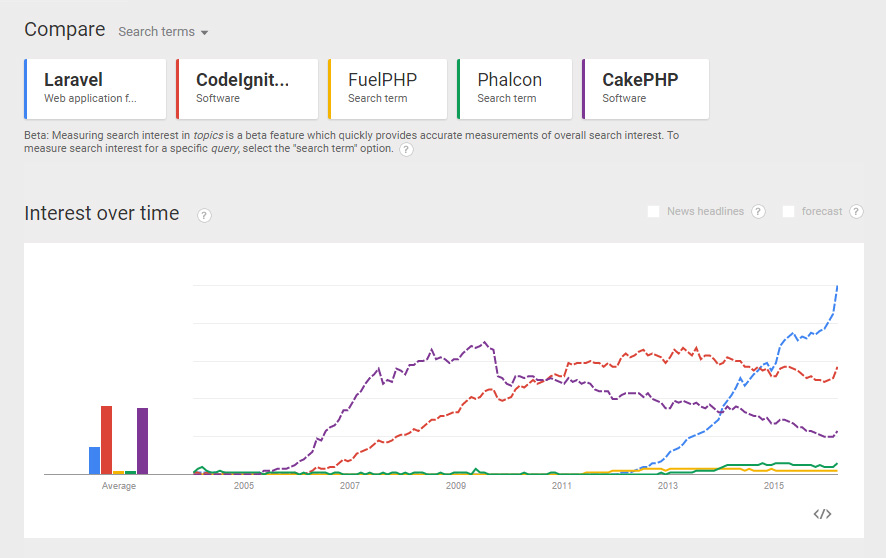
\includegraphics[width=120mm]{img/googletrends1.jpg}
  \centering
  \label{fig:googletrends Laravel 1}
\end{figure}
 
\begin{figure}[!ht]
 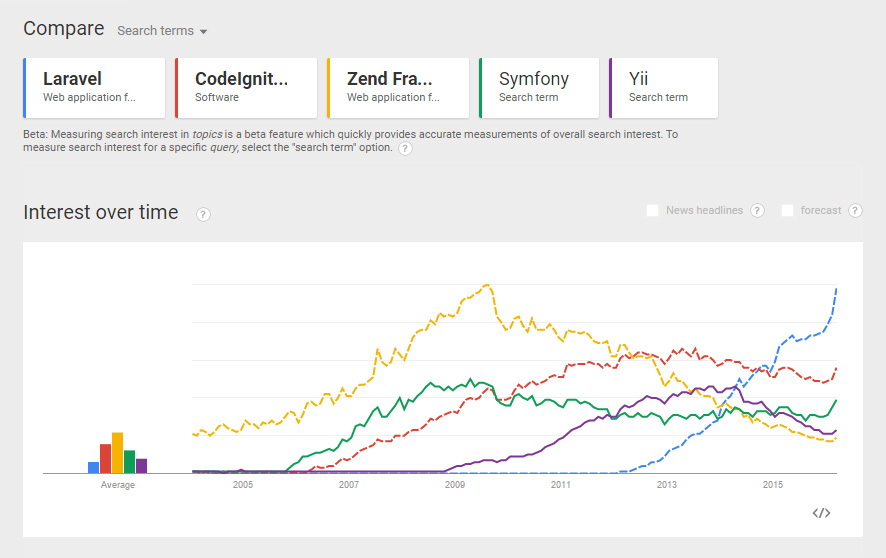
\includegraphics[width=120mm]{img/googletrends2.jpg}
 \centering
 \caption{Google trends waarbij verschillende populaire PHP frameworks worden vergeleken. Laravel torent hoog boven de anderen uit.}
  \label{fig:googletrends Laravel 2}
\end{figure}

\pagebreak

\begin{figure}[!ht]
  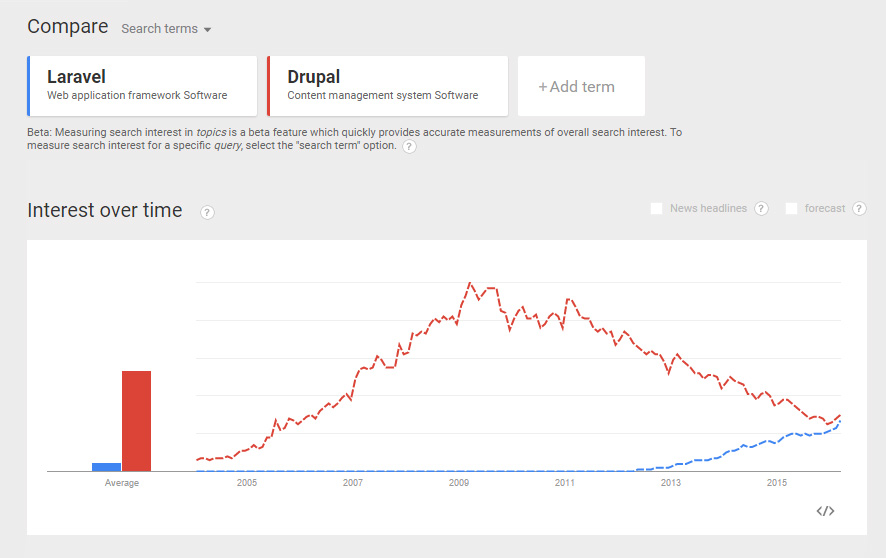
\includegraphics[width=\textwidth]{img/googletrends3.jpg}
   \centering
  \caption{Google trends vergelijking tussen Drupal en Laravel framework}
  \label{fig:googletrends Drupal 7 versus Laravel}
\end{figure}

\noindent
De grafiek op figuur: \ref{fig:googletrends Drupal 7 versus Laravel} toont puur informatief aan hoe het relatieve aandeel tussen Laravel en Drupal onderverdeeld is. Je kan hierop twee dingen waarnemen. Enerzijds dat Drupal een sterke negatieve trend vertoont, anderzijds dat Laravel sterk stijgt en bijna evenredig loopt met Drupal. Vermoedelijk zal het aandeel van Drupal binnenkort terug stijgen met de opkomst van Drupal 8. Ook al zijn deze twee systemen op deze manier moeilijk te vergelijken, toch geeft het een beeld weer van de populariteit.

\pagebreak
\noindent
Naast enkele zoektermen afgevuurd te hebben via Google trends biedt Github een zeer betrouwbare en interessante gegevensbron. Laravel staat op de eerste plaats als trending open source PHP framework (Figuur: \ref{fig:Github trending repos}). 

\begin{figure}[!h]
  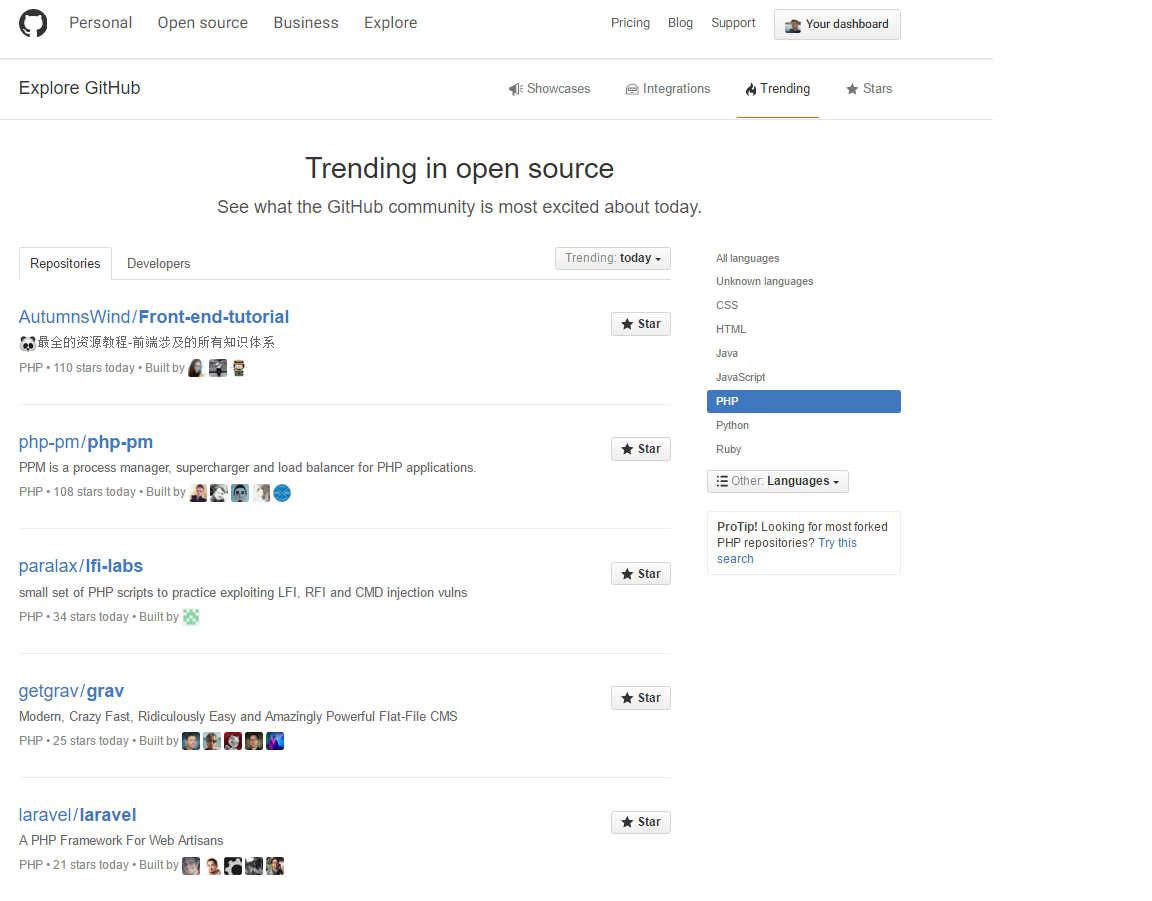
\includegraphics[width=\textwidth]{img/trending_repos.png}
  \centering
  \caption{Github trending repos}
  \label{fig:Github trending repos}
\end{figure}

\section{Wat maakt Laravel goed?}
Laravel kan webapplicaties aan van alle grootte en van alle complexiteit. Dit dankzij een aantal doorslaggevende voordelen dat het systeem biedt. Laravel is gebouwd om eenvoudig en snel te leren. Die leercurve wordt ondersteund door een goed uitgebouwde documentatie die neergeschreven staat als tutorials. Naast de standaard documentatie is er ook een aparte website die zich toelegt op video tutorials. Laracast.com stelt honderden video's ter beschikking. 

\section{Laravel CMS}
Laravel op zich is een PHP framework en geen CMS. Het is natuurlijk mogelijk om zelf een CMS te schrijven aan de hand van Laravel. Echetr,  dit is niet de doelstelling van dit werk. Daarom wordt er op zoek gegaan naar een bestaand CMS dat geschreven is via Laravel. Deze zoektocht geeft een lijst terug van een vijf-tal mogelijke CMS'en. Uit deze lijst wordt er slecht één CMS gekozen. Wegens de beperktheid van dit werk, is het onderzoeken van meerdere CMS'en niet mogelijk. 
\newline\newline
Om tot een keuze te komen werden de CMS'en onderworpen aan een aantal zaken. Zo werd gekeken welke zoekterm het beste naar voor kwam (Figuur: \ref{fig:Google Trends Laravel CMS}). Daaruit bleek duidelijk dat OctoberCMS als grootste speler naar voor komt. Naast zoektermen kan GitHub een zeer betrouwbare bron zijn voor allerhande ontwikkelprogramma's. Een zoekactie op 'Laravel CMS' leverde na filtering op aantal sterren, een grotendeels gelijklopend resultaat met Google Trends.
\newline\newline
OctoberCMS komt ook hier het beste naar voren. Meer nog, er is een duidelijke activiteit merkbaar bij dit systeem. De hoeveelheid en frequentie van updates, als ook het aantal 'Forks' ligt hoog. Personen die een 'Repository Fork' halen experimenteren of verbeteren het systeem. Forks worden in de meeste gevallen gebruikt om voorstellen tot aanpassingen te doen aan de projecteigenaar.
\newline\newline

\begin{figure}[!ht]
  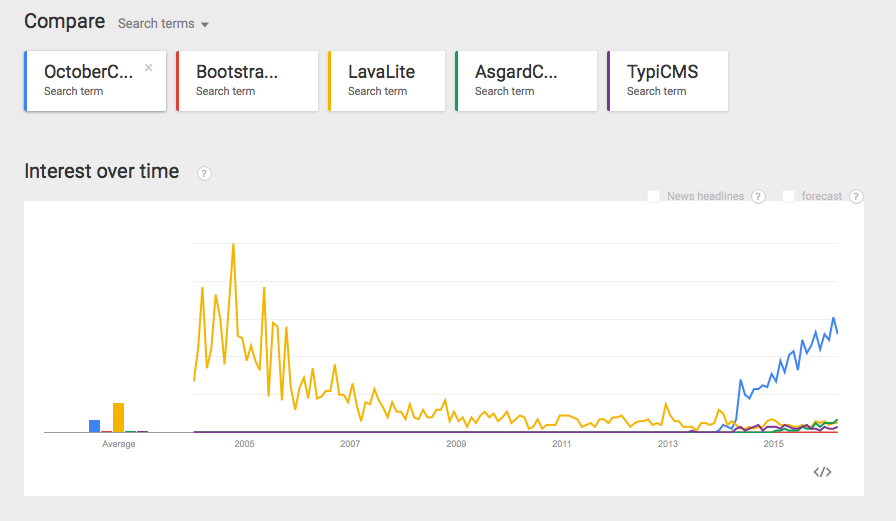
\includegraphics[width=100mm]{img/googletrends_laravelcms.png}
  \centering
  \caption{Google Trends voor Laravel CMS}
  \label{fig:Google Trends Laravel CMS}
\end{figure}

\begin{figure}[!ht]
  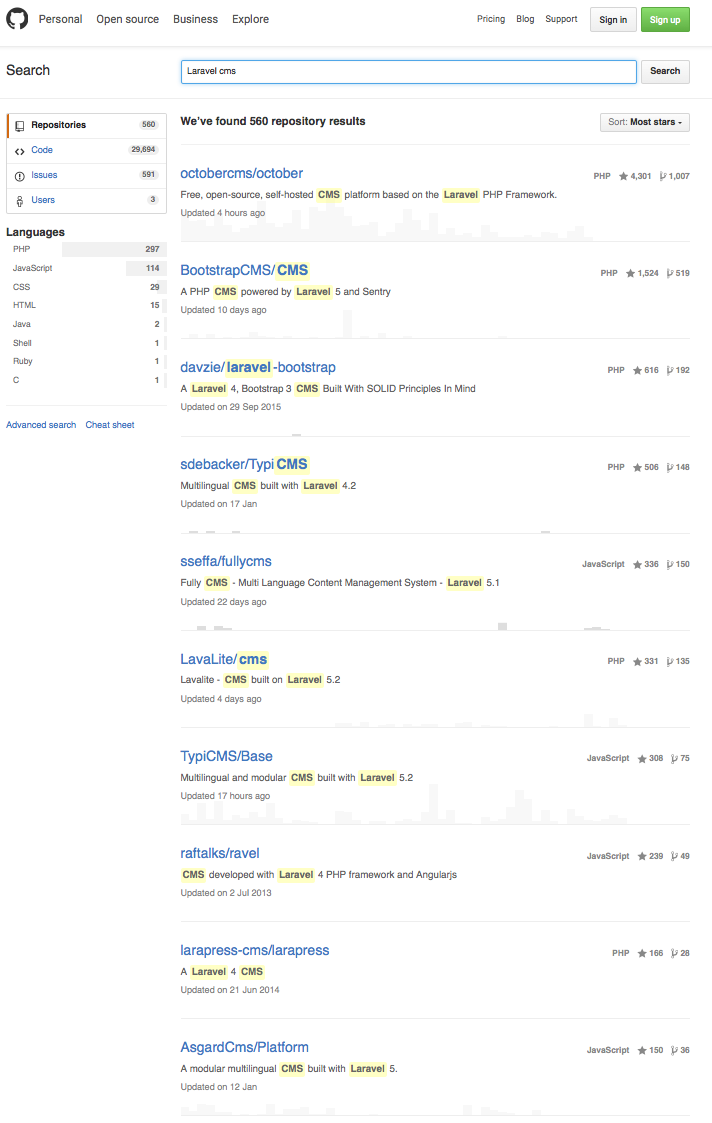
\includegraphics[width=70mm]{img/github_laravelCMS.png}
  \centering
  \caption{Github Laravel CMS}
  \label{fig:Github Laravel CMS}
\end{figure}

\noindent
Kortom, er leeft een community achter OctoberCMS, meer dan welk ander Laravel CMS. 

\section{OctoberCMS}
Elk CMS heeft zijn eigen specifieke eigenschappen en eigen systeem opbouw. De hoofdidee van dit CMS is terug te gaan naar de 'Basics', een licht systeem zonder complexe structuren en een duidelijke flow van begin tot einde. Dit systeem belooft een snelle leercurve waardoor de opstart van elk project binnen een aantal minuten klaar kan zijn. OctoberCMS op zich is geen framework, aangezien het als het ware op de schouders zit van een bestaand framework, Laravel. OctoberCMS zit op een hoger niveau en kan steunen op alle voordelen van het Laravel framework. Door te steunen op deze voordelen is het eenvoudiger en sneller ontwikkelen. 
\newline\newline
De hoofdgedachte die terug te vinden is op de website van OctoberCMS, is een duidelijk standpunt die ze innemen omtrent een CMS.
\newline\newline
\say{Clients don't build websites, developers do.}
\newline\newline
Een team dat deze gedachte als belangrijk ervaart, zal de pijnpunten die bijvoorbeeld Drupal heeft, teniet doen. Wanneer een CMS met de intentie is gebouwd om de eindgebruiker het roer van het schip te geven, zal de ontwikkelaar hoogstwaarschijnlijk snel stoten op het bereiken van het plafond van het systeem. De ontwikkelaar heeft zich niet volledig kunnen ontplooien in het project en grijpt terug naar een alternatief waar alles opnieuw uitgevonden moet worden. Dit heeft als gevolg dat ontwikkelen terug duurder wordt.
\newline\newline
Met OctoberCMS, met de doelgroep van ontwikkelaars, zullen deze sneller en goedkoper een project van a tot z opleveren.  Met kennis van HTML, CSS en PHP kan een standaard website ontwikkeld worden. Een grondige kennis van PHP is vereist wanneer de site bijkomende plugins nodig heeft. Plugins kunnen gezien worden als de belangrijkste elementen voor het uitbreiden van het OctoberCMS.
\newline\newline
OctoberCMS biedt een systeem met oog op ontwikkelen vanuit het perspectief van de ontwikkelaar, maar biedt ook een eenvoudig te beheersen systeem voor de eindgebruiker. Aanpassingen die de eindgebruiker doorvoert worden gedaan via de back-end in de browser. 